\chapter{Methodology} \label{chap:metodologia}

In this chapter, we intend to detail the pillar of our proposed methodology for our end-to-end framwork that aims to find the optimal bit-width for each layer of QNN while ensuring that the defined bit-widths satisfy robustness properties using SMT Theory of Fixed-Point Arithmetic.

From our work we aim to develop a end-to-end based on the work of Quadapter \cite{cai2025certified} for the synthesis of quantization and therefore find the optimal bit-width for each layer. However, we will extend it by integreting the SMT Theory of Fixed-Point Arithmetic like done in previous works \cite{baranowski2020smt, sena2021verifying, zhang2020qvip, huangEfficientVerificationQuantized2023, henzingerScalableVerificationQuantized2022} to check if the defined constrains are satisfied by the quantization strategy. Whether not, the counterexample will be used to refine the quantization.

The work methodology can be described in the diagram shown in Figure~\ref{fig:diagrama_metodologia}. From it, we can divide the work into two sub-problems. The first problem would be to find out the minimum bit-width and it will be described in Section~\ref{sec:bit_width}. The second problem would be to verify whether the defined bit-widths satisfy the required properties and it will be described in Section~\ref{sec:verificacao}.  

\begin{figure}[H]
    \centering
    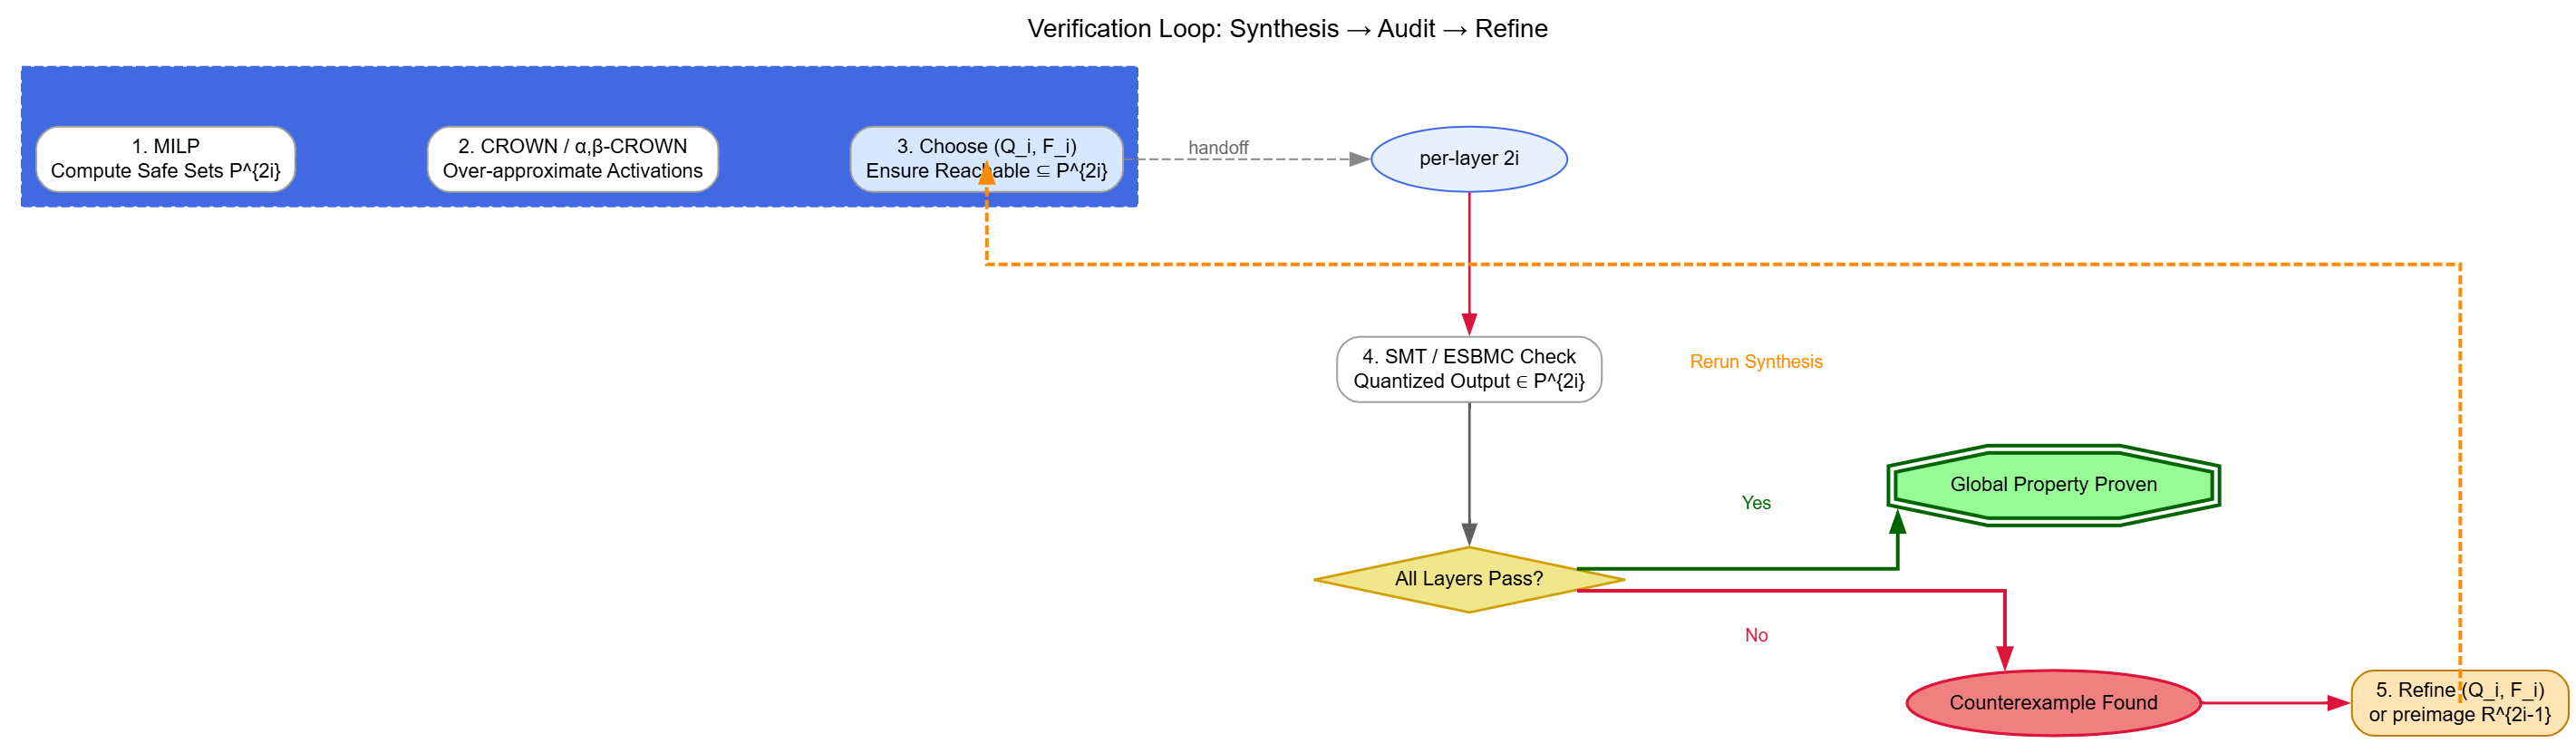
\includegraphics[width=1\textwidth]{figuras/3-metodologia/flowDiagram.png}
    \caption{Proposed Methodology Diagram}
    \label{fig:diagrama_metodologia}
\end{figure}


% Title find through Synthesis the title of section where the bit-width will be defined
\section{Finding the Minimum Bit-width for Each Layer}\label{sec:bit_width}
There are several works that focus on finding the optimal bit-width for each layer of a neural network \cite{sena2021verifying}. Sena et al. proposed a Bit Search Module (BSM) which uses a counter-example guided approach to find the optimal bit-width. The BSM proposes the usage of genetic algorithms that iteractively proposes a vector of bit-widths for each layer and then uses a verifier to check if the defined constrains are satisfied. If not, the counter-example is used to refine the bit-widths. The process is repeated until a satisfactory solution is found or a limit of iteractions is met.



Given a DNN $N$ with $2d$ layers. 

Our objective would be to find the minimum bit-width for each layer such that the quantized  network $\hat{N}$ preserves a desired property, such as adversarial robustness or the absence of backdoors.

The vector of bit-widths for each layer if defined as $\mathbf{b} = (b_1, b_2, \ldots, b_{2d})$, where $b_i$ is the bit-width for layer $i$. The quantized network $\hat{N}$ is obtained by applying a quantization function $Q_{b_i}$ to the weights and activations of each layer $i$.



\section{Verification of QNN Bit-width using Bit-precision SMT-Solving}\label{sec:verificacao}




\subsection{Refine}

\begin{comment}
    
    \section{Problem}
    
    ANN are widely used in various applications, but their computational and memory resource demands are high \cite{amir2021smt, han2020understanding, abdi2021counterexample, song2023qnnrepair}. Quantization is a crucial technique to mitigate this problem by reducing the bit-width (from 32-bit floating-point to 8-bit integers or even binary) used to represent weights, biases, and activations, making networks more efficient on embedded and low-power devices \cite{amir2021smt, han2020understanding,song2023qnnrepair, abdi2021counterexample, Cai2020Certified}.

    However, quantization introduces an "implementation gap" \cite{cordeiro2025neuralnetworkverificationprogramming}. Most formal verification techniques for neural networks (such as Reluplex and Marabou) assume that networks operate with real-number arithmetic \cite{katz2017reluplex,amir2021smt}. In contrast, actual hardware implementations use finite-precision arithmetic, such as low-precision floating-point or, more frequently, fixed-point \cite{han2020understanding}. This discrepancy means that the safety and correctness guarantees obtained on ideal models may not hold for the deployed neural network \cite{abdi2021counterexample}.

    Furthermore, quantization, while beneficial for efficiency, can degrade accuracy and, more critically, compromise desired safety and correctness properties, such as adversarial robustness (resistance to small input perturbations that change the classification) and the absence of backdoors (intentionally inserted vulnerabilities). Existing work on QNN verification generally focuses on post-hoc analyses; that is, they verify a network after it has been quantized \cite{abdi2021counterexample,Cai2020Certified}.
    
\section{Proposed Approach}
This work proposes the development of a framework for the certified synthesis of quantization strategies that guarantee the preservation of desired properties after quantization, directly addressing finite-precision arithmetic. This differs from post-hoc approaches and quantization techniques that focus solely on accuracy.

\textbf{Synthesis of Quantization Strategies (Inspired by Quadapter):}
The work Quadapter is the first to propose the synthesis of certified quantization strategies \cite{Zhu2021Quadapter,Cai2020Certified}. Its central idea is to compute the pre-image of each layer with respect to the desired output region and then identify the minimum bit-width for each layer, ensuring that the quantized layer's reachable region remains within that pre-image.

This work would extend this line of research by focusing on the incorporation of fixed-precision arithmetic during the synthesis process. This is not the primary focus of Quadapter in its current state, which, while dealing with realistic quantization representations, does not yet formally incorporate the nuances of fixed-point arithmetic during verification.

\textbf{Formal Integration of the SMT Theory of Fixed-Point Arithmetic:}
A fundamental contribution would be the use of the SMT Theory of Fixed-Point Arithmetic, as formalized by \cite{baranowski2020smt}. This theory provides a rigorous formalization for fixed-point operations, including rounding modes (roundUp, roundDown) and overflow modes (saturation, wrapAround).

The proposal is to integrate this formal theory into the pre-image calculation and quantization procedures of the synthesis framework. This would allow the synthesized quantization strategies to be certified for the specific finite precision of the hardware, ensuring that properties hold even with the effects of rounding and overflow. The methods of \cite{baranowski2020smt} already include decision procedures for this theory, via both bit-vectors and reals, which is essential for a verifier. They themselves demonstrate a case study using this theory to verify QNNs.

This would more robustly solve the "implementation gap," as the formal guarantees would be directly on the behavior of fixed-point arithmetic, not just a real-number approximation.

\textbf{Pre-image Calculation with Fixed-Point Semantics:}
Quadapter uses a method based on Mixed-Integer Linear Programming (MILP) to compute under-approximations of the pre-image. This work would adapt this MILP formulation to precisely reflect fixed-point operations (including rounding and overflow) instead of just real numbers. This would ensure that the calculated pre-image already accounts for the effects of finite precision.

\textbf{Bit-Precise Verification in Progressive Quantization:}
In Quadapter's progressive quantization algorithm, the verification step $\left(\gamma(\hat{A}_{2i}) \subseteq P_{2i}\right)$ \textcolor{red}{(Still have to add the math theory)} compares the quantized reachable region with the pre-image. The proposal is to use formal SMT-based fixed-point reasoning (potentially through backends like ESBMC) to perform this verification in a bit-precise manner \cite{esbmc2025}. This would mean that the inclusion of the quantized reachable region within the pre-image would be verified considering the exact rules of fixed-point arithmetic.

QNN verification is a PSPACE-hard problem, and scalability is a known challenge for all verifiers (e.g., Marabou, Reluplex, CEG4N). Even Quadapter faces timeouts in pre-image calculations.

\textbf{Adaptive/Dynamic Quantization:} While Quadapter synthesizes per-layer bit-widths, this research could explore how to fine-tune precision (e.g., different precisions within a layer, as discussed by \cite{han2020understanding,abdi2021counterexample}) in a verification-guided manner to minimize bit requirements without losing properties, seeking a balance that optimizes verifier performance.

\section{Experimental Methodology}

To empirically validate the certified quantization synthesis methodology proposed in this dissertation, a meticulous selection of public benchmarks, widely recognized in the formal verification of neural networks community, will be used. The choice of benchmarks was designed to ensure a comprehensive evaluation, covering a variety of network architectures, application domains, and safety properties. The basis for this selection includes the challenges proposed by the Neural Network Verification Competition (VNN-COMP) and the test suites made available in foundational works in the field \cite{cordeiro2025neuralnetworkverificationprogramming,abdi2021counterexample}.

The evaluation suite will be composed of the following main components. First, for image classification tasks, we will use models trained on the \textbf{MNIST}, \textbf{CIFAR-10}, and \textbf{Fashion-MNIST} datasets. These range from simple, few-layer networks, ideal for scalability analysis, to complex architectures like LeNet, VGGNet, ResNet-18, and MobileNetV2, allowing the framework to be evaluated in realistic scenarios \cite{han2020understanding, qnsong2023qnnrepairCai2020Certified}. Second, for the domain of safety-critical systems, the \textbf{ACAS Xu} benchmark will be central, given its status as the de facto standard for verifying airborne controllers \cite{katz2017reluplex}. Finally, to enable agile prototyping and debugging, smaller-scale models will be employed, such as those used in the \textbf{fairness} case studies with tabular data and the fixed-point quantized \textbf{Cart-Pole} controller \cite{baranowski2020smt}. The primary focus of the certified synthesis will be the preservation of \textbf{adversarial robustness}, a critical and extensively studied property, with the possibility of extension to other formal specifications.


\section{Expected Contributions}
An innovative framework and methodology for the certified synthesis of bit-precise quantization strategies for neural networks, offering formal guarantees that extend to finite-precision implementations.

A formal and empirical demonstration of the impact of fixed-point arithmetic semantics on the preservation of properties during quantization.

Significant scalability improvements for the verification and synthesis of larger and deeper QNNs by combining the power of SMT with fixed-point theory and optimization techniques.

An extension of the approach to guarantee other critical properties, such as adversarial robustness and the absence of backdoors, beyond the functional equivalence already explored in other contexts (e.g., CEG4N) \cite{abdi2021counterexample}.

This work would fill a critical gap in the research, providing a rigorous foundation for the deployment of safe and reliable neural networks in resource-constrained critical systems.


\chapter{Rascunho}

A pré-imagem (preimage) é um conceito fundamental em diversos trabalhos sobre verificação e síntese de redes neurais quantizadas.
O que é a Pré-imagem?
Formalmente, para uma função $f$ e um conjunto de saída $Y$, a pré-imagem $f^{-1}(Y)$ do conjunto de saída $Y$ para $f$ é o conjunto de todas as entradas $x$ para as quais $f(x) \in Y$. No contexto de redes neurais, uma sub-aproximação (under-approximation) da pré-imagem é um conjunto $P$ tal que $P \subseteq f^{-1}(Y)$.
Em um DNN (Deep Neural Network) $N$ com $2d$ camadas, uma pré-imagem sub-aproximada das regiões de saída $O$ para o DNN $N$ é um conjunto $P = {P_{2i} \mid i \in [d-1]}$, onde para cada $i \in [d-1]$, $P_{2i} \subseteq N^{-1}{[2i+1:2d]}(O)$. Intuitivamente, $P{2i}$ (ou $P_{2i,j}$) é a pré-imagem da camada de ativação $f_{2i+1}$ (ou neurônio $x_{2i+1,j}$) em relação à região de saída $O$. As pré-imagens das camadas afins são excluídas, pois basta considerar as pré-imagens das camadas de ativação para calcular as larguras de bits das camadas afins.
Propósito da Pré-imagem
A pré-imagem é utilizada para garantir que as propriedades desejadas (como robustez adversarial e ausência de backdoors) sejam preservadas após a quantização. A ideia é que, independentemente das configurações de quantização das primeiras $2i$ camadas, a propriedade é sempre mantida na rede neural quantizada resultante, desde que a região alcançável da camada quantizada permaneça dentro da pré-imagem correspondente. Isso permite derivar uma estratégia de quantização para toda a rede que preserva a propriedade desejada.
Como a Pré-imagem é Calculada?
O cálculo da pré-imagem é um passo crucial no método Quadapter para a síntese de estratégias de quantização certificadas. Ele envolve os seguintes passos:
1. Propagação Reversa (Backward Propagation):
    ◦ As pré-imagens são calculadas recursivamente da camada de saída para as camadas de entrada. O processo começa definindo $P_{2d} = O$ (a região de saída).
    ◦ Para cada camada de ativação $f_{2i+1}$, a função UnderPreImage é invocada para propagar a pré-imagem $P_{2i+2}$ para a camada de ativação precedente, retornando uma pré-imagem aproximada $P_{2i}$ tal que $P_{2i} \subseteq N^{-1}{[2i+1:2i+2]}(P{2i+2})$.
    2. Método Baseado em MILP (Mixed Integer Linear Programming):
    ◦ Para computar a pré-imagem (especificamente, uma sub-aproximação), utiliza-se um método baseado em MILP.
    ◦ Para uma pré-imagem $P_{2i+2}$ e os elementos abstratos $A_{2i}$ da camada $f_{2i}$, constrói-se um problema de maximização com a função objetivo $\chi_{2i}$ (uma variável de escala) sujeita às restrições de que o template $T_{2i}$ da pré-imagem $P_{2i}$ esteja contido em $N^{-1}{[2i+1:2i+2]}(P{2i+2})$.
    ◦ As transformações afins e as funções de ativação (como ReLU) são codificadas precisamente como restrições lineares dentro do problema MILP.
    3. Adaptação do DeepPoly:
    ◦ O método adapta o domínio abstrato do DeepPoly para representar a pré-imagem. O DeepPoly calcula limites inferiores e superiores simbólicos para a saída de cada neurônio, que são combinações lineares das variáveis de entrada.
    ◦ O template da pré-imagem $P_{2i}$ é definido como uma conjunção de expressões que escalam os elementos abstratos do DeepPoly da camada $f_{2i}$ usando uma variável de escala $\chi_{2i}$.
4. Desafios e Alternativas:
    ◦ O cálculo exato da pré-imagem é impraticável devido à sua complexidade exponencial.
    ◦ Existem métodos alternativos baseados em abstração (ABS), que tendem a obter valores significativamente menores para as variáveis de escala nas camadas iniciais, embora exijam menos tempo de computação. No entanto, valores maiores para as variáveis de escala nas camadas iniciais são preferíveis para o sucesso do processo de quantização subsequente.
    ◦ Outras abordagens, como a abstração inversa usando interpolantes simbólicos, também enfrentam problemas de escalabilidade.
Papel na Quantização Certificada
Após o cálculo da pré-imagem, a estratégia de quantização é sintetizada em um processo de "quantização progressiva" (forward quantization). Nesta etapa, para cada camada, o algoritmo busca uma configuração de quantização com a menor largura de bits possível. A verificação principal é que a região alcançável (reachable region) da camada quantizada (calculada usando DeepPoly) deve estar estritamente contida na pré-imagem calculada para essa camada. Essa inclusão é crucial para garantir que a propriedade desejada seja mantida.
Em resumo, o cálculo da pré-imagem, via métodos MILP e adaptações do DeepPoly, atua como um "guia" reverso para determinar as restrições de precisão em cada camada, assegurando que a quantização não comprometa as garantias formais do comportamento da rede neural.



No capítulo de metodologia, detalho a proposta de um framework para a síntese certificada de redes neurais quantizadas. A abordagem se baseia no cálculo da pré-imagem de cada camada para garantir que propriedades de segurança, como a robustez, sejam preservadas após a quantização. A principal inovação é a integração da aritmética de fixed-point no processo de síntese, permitindo uma verificação bit-precisa. 
\end{comment}



%% Algumas ideias

\begin{comment}
    
    \\ Ideia para pesquisa
    Invés de usar apenas MILP, usar SMT junto ao MILP, como um algoritmo híbrido. O MILP seria responsável por encontrar a pré-imagem e calcular os melhores bit-widths, enquanto SMT seria responsável por verificar se a quantização está correta e representando a aritmética de ponto fixo. Caso contrário, um contra exemplo seria retornado e usado para refiniar a quantização.

    \\ Otimizacao
    Aprimarar trocando (DeepPoly) por (\alpha-beta-CROWN) e usar BaB consicente do bit-width.

    \\ 
    \cite{giacobbe2020how} proposed to  verify many-bit quantized neural network by encoding their semantics and specifications into quantifier-free bit-vector  SMT (QF_BV) formulas.


    \\ Counter Example Guided Quantization for Neural Networks
    \cite{abdi2021counterexample} proposed a CEG4N algorithm that is divided into 3 modules: the first module is responsible for finding the optimal bit-width for each layer with counter-examples as input. The second module, after the bit-widths are defined, encodes the NN and QNN into a format third module can handle. The format is based on ONNX; NN and QNN are converted separately. The third module is a verifier that checks if property holds.


\end{comment}